% %%% Time-stamp: <2023-11-11 22:31:14 vladimir>
% %%% Copyright (C) 2019-2023 Vladimir G. Ivanović
% %%% Author: Vladimir G. Ivanović <vladimir@acm.org>
% %%% ORCID: https://orcid.org/0000-0002-7802-7970

\chapter{Discussion}%
\label{ch:discussion}%
\noindent\bigskip%

This chapter addresses this dissertation's research question:
\medskip%
\begin{quote}\OnehalfSpacing
  Has Rocketship structured itself to earn a return for its founders and investors, focusing especially on its real estate transactions?
\end{quote}
The chapter looks more closely at the research question and summarizes the key findings of the research. It then discusses what kind of evidence would confirm or disconfirm the research question. It looks at three well-known approaches to making arguments for or against a proposal or policy and uses those approaches to make the case that Rocketship has in fact organized itself to make money and that real estate is the vehicle it uses. The two final sections discuss what policy issues are raised during the examination of the data and the evidence, what further research is warranted. Lastly, this dissertation makes a brief conclusion.

\section{The Research Question}%
\label{sec:research-question}\indent%

The research question really is asking three questions:
\begin{enumerate}
  \item Has Rocketship structured itself to make money?
  \item If so, is real estate the vehicle that Rocketship uses to make money?
  \item Is this Rocketship's intent?
\end{enumerate}

\section{Key Findings}%
\label{sec:summary-key-findings}\indent%

\section{Arguments Which Answer the Research Question}%
\label{sec:appr-answ-rese-quest}\indent%

\subsection{Rappaport's Rules}%
\label{sec:rappaports-rules}\indent%

Anatol Rapoport, a [mathematical] game theorist, proposed four rules that seek to increase understanding and avoid defensive responses. \citefirstlastauthor{Dennett2013} reformulated them in his book \citetitle{Dennett2013} \parencite{Dennett2013}:
\begin{enumerate}[topsep=0.3\baselineskip,itemsep=0.25\baselineskip]
  \item You should attempt to re-express your target’s position so clearly, vividly, and fairly that your target says, “Thanks, I wish I’d thought of putting it that way.”
  \item You should list any points of agreement (especially if they are not matters of general or widespread agreement).
  \item You should mention anything you have learned from your target.
  \item Only then are you permitted to say so much as a word of rebuttal or criticism.
\end{enumerate}
\medskip

Here, in Rocketship's case, their argument might go along the following lines:
\begin{enumerate}[topsep=0.3\baselineskip,itemsep=0.25\baselineskip]
  \item Public schools in areas of poverty, for whatever reason, don't educate children well, and they educate children of color especially poorly. We (Rocketship) aim to change this by a combination of focus, targeted intervention, and technology. We are focused on doing whatever it takes to raise the educational attainment of our students, and we focus day in and day out on this one goal. Our pedagogy has two major aspects: We monitor and target with specialize intervention students who are not doing as well as we would like, and we use technology (computer-aided instruction) to tailor instruction to a specific child's needs.
  
  We believe that, by controlling our facilities, we can remove a serious distraction that comes with sharing facilities with a public school district. Not only are we not beholden to the whims of the public school district, but we don't have to spend time preparing year after year a Proposition 39 facilities request. We are never embroiled in petty disputes about interactions between public school students and our students because they never arise. Our results speak for themselves. All of our schools do better than their surrounding district and do better than the California average.
  \item I agree that some public school districts have failed in their primary duty to educate children, but staying the course is not an option because doing the same thing over and over and expecting different results is not likely to be successful, now or ever.
  I also agree that providing separate facilities for children rather than forcing them to share is more likely to be successful than otherwise. Being able to control the teaching environment brings stability the classroom.
  \item Starting and operating a charter school is not for the faint of heart. Funding for both operation and for facilities is hard to come by, and must be procured before a single student arrives on campus. Facilities need to be constructed or modified well before classes begin. Children need to be enrolled, and parents need to be persuaded to help out. Juggling priorities, contingencies, and expectations is a full-time task, and it shows when the topics of board committee (executive, business, achievement, development) meetings are looked at.
    \item However, even given the truthfulness of the items 1–3 above, there are some areas where criticism, some of it severe, is warranted.
    \begin{itemize}[topsep=0.125\baselineskip,itemsep=0.25\baselineskip]
      \item Rocketship spends an inordinate amount of time on topics that are not academic in focus. One can see this in the topic areas of its board committees, where only one of four has to do with academic achievement.
      \item Rocketship short-changes current students in order to create future students by allocating 20\% of revenue to facilities. Although this is  legal, I suspect that the California Legislature did not expect one charter school begetting another and so on when they created the legislation which allowed charter schools to exist, just as they didn't anticipate the damage that for-profit charter school chains or virtual charter schools would do.
      The percentage of revenue that Rocketship spends on administration (i.e. management), is unusually high at 15\%. Public school districts are limited to 9\%. So, right off the top, 35\% of revenue is siphoned off and does not go directly to educating children.
      \item Teachers at Rocketship schools in Santa Clara county have much less experience and are paid substantially less than, say, teachers in the San José Unified School District. If we believe that teachers are a key factor in delivering a quality education, then what kind of teachers Rocketship hires and how much it pays them are important determinants of the quality of the teaching staff and hence how well Rocketship educates its children.
      \item Rocketship has seriously exaggerated how well its students do compared to public school students. The size of the discrepancy, 4× to 5× larger than what was reported in the literature, seems to indicate a certain amount of desperation to convince people that Rocketship is both committed to ``eliminating the achievement gap in our lifetime'' and successful at it.\\
      According to the latest \citetitle{SCCOE2014}, comparing the percentage of Rocketship students who ``met/exceeded standards'' on the Smarter Balanced Summative Assessments (SBAC) test in English Language Arts (ELA) during the 2021-22 school year, only a single Rocketship school (out of eight Santa Clara County authorized schools) did better than public school students in Santa Clara County. In Mathematics, the number of schools who did better was actually less than one; it was zero.\\
      Moving on to comparing how Rocketship schools did against state public schools, only one school exceeded the state average in ELA—by a single percentage point—and five exceeded the state average in Mathematics. Granted, these results are not as bad as ACE Empower that managed only 19\% met or exceeded standards in ELA and 11\% in Mathematics, but for a chain of schools whose goal is to close the achievement gap, Rocketship's scores are not encouraging \parencite{SCCOE2014}.\\
      Also discouraging is the trend in the last five years. In five schools, the percent met/exceeded has fallen in ELA and all but one have fallen in Mathematics. However, a deeper dive into the scores is needed to determine if this because parents with children who were not doing as well as hoped for enrolled and thus brought the average scores down, or whether this is truly a reflection on the effectiveness of Rocketship's pedagogy. More honesty and transparency and less of the cult-like chanting at the start of a school day would be welcome.
      \item Rocketship's policy of owning its facilities has led to over \$185M\footnote{This figure is for all Rocketship schools, i.e. those in  California, Tennessee, Wisconsin, Washington, D.C. and Texas.} in debt, which comes to roughly \$32K per child. At 3\% per annum, that's another \$5.4M that is not going toward educating children.
    \end{itemize}
\end{enumerate}

\subsection{A Toulmin Argument}%
\label{sec:toulmin-arguments}\indent%

Stephen Toulmin was a British philosopher interested in moral reasoning. He developed a method for making practical arguments where ethics and morality played a role. His method has six components, of which the first three are those most commonly seen.
\begin{enumerate}[topsep=0.3\baselineskip,itemsep=0.25\baselineskip]
  \item Claims are statements, conclusions which must be justified.
  \item Evidence (facts, data) are used to provide the basis for making the claim.
  \item Warrants are the connection between the claim and the evidence which backs up the claim.
  \item Backings buttresses a warrants.
  \item Rebuttals are counter-arguments, made in advance, to potential objections.
  \item Qualifiers express the degree of certainty about the claim.
\end{enumerate}

\prettyref{fig:toulmin-arg} below diagrams the relationship between the parts of a Toulmin argument where rebuttals have been substituted for reservations.

\begin{figure}[ht]
  \caption{The Toulmin Argument Schema}%
  \label{fig:toulmin-arg}%
  \copyrightbox[b]{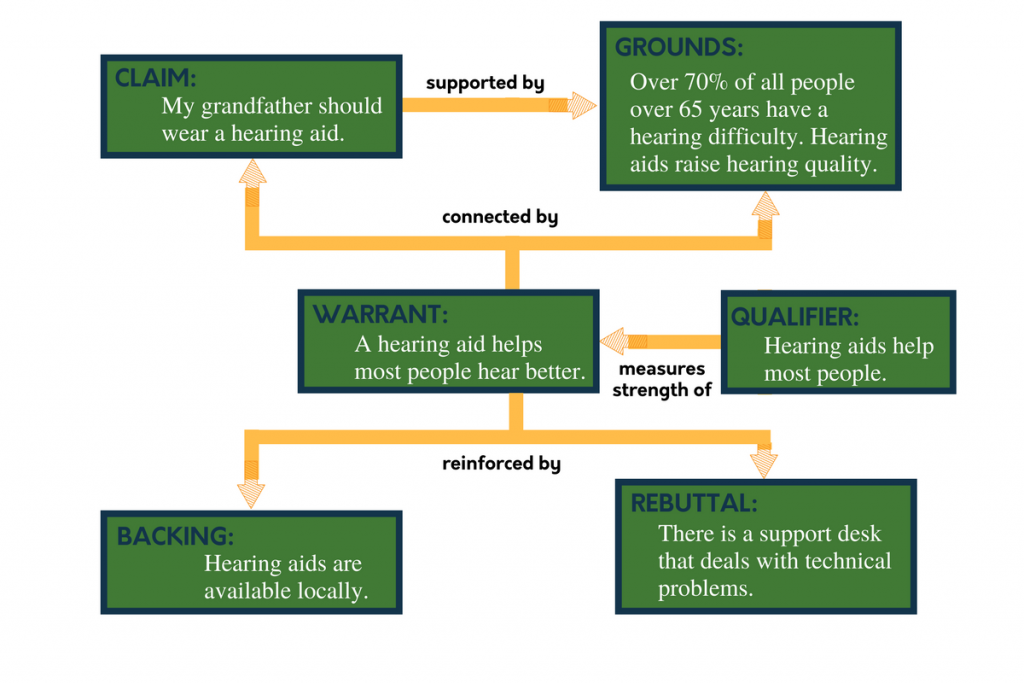
\includegraphics[scale=0.5]{The Toulmin Argument Schema}}{“Toulmin Argument,” Kalyca Schultz, Virginia Western Community College, CC-BY-SA in “Toulmin Argument Model” by Liza Long, Amy Minervini, and Joel Gladd is licensed under CC BY-NC-SA 4.0}
\end{figure}

Using the Toulmin schema, I \textit{claim} that Rocketship is structured to return an as yet unrealized profit to founders and investors, and that real estate is the mechanism they are using to turn a profit. The \textit{grounds} on which I base this claim are
\begin{itemize}
  \item Rocketship's primary focus is not on academic success, but on acquiring real estate. Right from the beginning, Rocketship separated the financing, acquisition, and operation of their facilities from the running of a school; they borrowed heavily and made extensive use of government programs to fund their real estate projects.
  \item Simply judging by the number of board committees devoted to non-academic topics, Rocketship leadership has spent most of their time on real estate issues.
  \item Rocketship has not availed itself (except in one instance) of alternative ways of acquiring necessary facilities. They have not used Proposition 39 to obtain classrooms and fields from a school's home district. They have not tried to convert commercial office space into classrooms. They have not modified existing buildings to serve as schools or classrooms.
\end{itemize}
The \textit{warrant} that connects my claims to the grounds for making my claims is colloquially expressed by the phrase, ``Where there is smoke, there is fire.'' By looking at what Rocketship does or where it spends its time, one can identify what Rocketship thinks is important. By looking at its finances, one can identify where is spends it money. Both of these point to profit and to real estate.

\begin{comment}
  Rocketship's and Launchpad Development's Articles of Incorporation do not include a strong, clear statement that no individual is to profit from their activities like Summit Public Schools' does.
\end{comment}

\section{Answering the Research Question}%
\label{sec:answ-rese-quest}\indent%

\section{Public Policy Issues}%
\label{sec:publ-policy-chang}\indent%

\section{Areas for Future Research}%
\label{sec:issu-future-rese}\indent%

\section{Conclusion}%
\label{sec:conclusion}\indent%


%%% Local Variables:
%%% mode: latex
%%% TeX-master: "Rocketship_Education-An_Exploratory_Public_Policy_Case_Study"
%%% End:
